\documentclass[12pt,a4paper,titlepage]{article}
\usepackage{License_style}
\usepackage{pdfpages}
\usepackage{eso-pic}

  
\begin{document}
\pagenumbering{gobble}


\numberwithin{lstlisting}{section}


% TITLE
\begin{titlepage}
\selectlanguage{romanian}

\newcommand{\HRule}{\rule{\linewidth}{0.5mm}} % Defines a new command for the horizontal lines, change thickness here

\center

Ministerul Educației al Republicii Moldova\\ % Name of your university/college
Universitatea Tehnică a Moldovei \\% Name of your university/college
Facultatea de Calculatoare, Informatică și Microelectronică\\
Filiera Anglofonă "Computer Science"\\


\vspace{6cm}

\begin{center}
\LARGE \textbf{Views in SQL}\\
\vspace{0.6cm}
Course Thesis\\
\vspace{0.6cm}
Baze de Date și Cunoștințe
\end{center}
\vspace{4cm}


\hfill Student: Vlas Mihai, FAF-141\\
\vspace{0.2cm}
\hfill Conducător: Irina Cojanu\\
\vspace{0.2cm}




% If you don't want a supervisor, uncomment the two lines below and remove the section above
%\Large \emph{Author:}\\
%John \textsc{Smith}\\[3cm] % Your name

%----------------------------------------------------------------------------------------
%	DATE SECTION
%----------------------------------------------------------------------------------------
\vfill % Fill the rest of the page with whitespace
\begin{center}
Chișinău 2017
\end{center}


\end{titlepage}
\selectlanguage{english}


\cleardoublepage


\tableofcontents

\newpage

\pagenumbering{arabic}
\setcounter{page}{4}
\setcounter{secnumdepth}{4}

\addtocontents{toc}{\protect\thispagestyle{empty}} % no page number on the table of contents page
\cleardoublepage


%LISTA FIGURILOR. Este recomandabila daca in text ai peste cel putin 10-15 FIGURI
%\listoffigures
%\addcontentsline{toc}{section}{List of figures}
%\clearpage

%LISTA TABELELOR. Este recomandabila daca in text ai peste cel putin 10-15 tabele
%\listoftables
%\addcontentsline{toc}{section}{List of tables}
%\clearpage

%INTRODUCERE
%\setcounter{page}{17} 
\phantomsection
\addcontentsline{toc}{section}{Introduction}
\section*{Introduction}
\phantomsection

\textbf{SQL} stands for Structured Query Language, is a domain-specific language used in programming and designed for managing data held in a relational database management system (RDBMS), or for stream processing in a relational data stream management system. Originally based upon relational algebra and tuple relational calculus, SQL consists of a data definition language, data manipulation language, and data control language. The scope of SQL includes data insert, query, update and delete, schema creation and modification, and data access control. Although SQL is often described as, and to a great extent is, a declarative language (4GL), it also includes procedural elements.

SQL was one of the first commercial languages for Edgar F. Codd's relational model, as described in his influential 1970 paper, "A Relational Model of Data for Large Shared Data Banks." Despite not entirely adhering to the relational model as described by Codd, it became the most widely used database language.

SQL became a standard of the American National Standards Institute (ANSI) in 1986, and of the International Organization for Standardization (ISO) in 1987. Since then, the standard has been revised to include a larger set of features. Despite the existence of such standards, most SQL code is not completely portable among different database systems without adjustments.
The SQL language is subdivided into several language elements, including:

Clauses, which are constituent components of statements and queries. (In some cases, these are optional.)
Expressions, which can produce either scalar values, or tables consisting of columns and rows of data
Predicates, which specify conditions that can be evaluated to SQL three-valued logic (3VL) (true/false/unknown) or Boolean truth values and are used to limit the effects of statements and queries, or to change program flow.
Queries, which retrieve the data based on specific criteria. This is an important element of SQL.
Statements, which may have a persistent effect on schemata and data, or may control transactions, program flow, connections, sessions, or diagnostics.
SQL statements also include the semicolon (";") statement terminator. Though not required on every platform, it is defined as a standard part of the SQL grammar.
Insignificant whitespace is generally ignored in SQL statements and queries, making it easier to format SQL code for readability.
\clearpage
\cleardoublepage

% CAPITOLUL 1
\section{Views in SQL}
\phantomsection

In SQL, a view is a virtual table based on the result-set of an SQL statement.
A view contains rows and columns, just like a real table. The fields in a view are fields from one or more real tables in the database.
You can add SQL functions, WHERE, and JOIN statements to a view and present the data as if the data were coming from one single table.
A view can contain all rows of a table or select rows from a table. A view can be created from one or many tables which depends on the written SQL query to create a view.\\
Views, which are a type of virtual tables allow users to do the following:\\
•	Structure data in a way that users or classes of users find natural or intuitive.\\
•	Restrict access to the data in such a way that a user can see and (sometimes) modify exactly what they need and no more.\\
•	Summarize data from various tables which can be used to generate reports.\\
\\
Besides the standard role of basic user-defined views, SQL Server provides the following types of views that serve special purposes in a database:\\
{\large • Indexed Views:}
An indexed view is a view that has been materialized. This means the view definition has been computed and the resulting data stored just like a table. You index a view by creating a unique clustered index on it. Indexed views can dramatically improve the performance of some types of queries. Indexed views work best for queries that aggregate many rows. They are not well-suited for underlying data sets that are frequently updated.\\
{\large • Partitioned Views:}
A partitioned view joins horizontally partitioned data from a set of member tables across one or more servers. This makes the data appear as if from one table. A view that joins member tables on the same instance of SQL Server is a local partitioned view.\\
\\
{\large • System Views:}
System views expose catalog metadata. You can use system views to return information about the instance of SQL Server or the objects defined in the instance. For example, you can query the sys.databases catalog view to return information about the user-defined databases available in the instance.\\
\\
\clearpage
There are several actions that we can do with views in SQL:\\
1) \textbf{Create View}\\
2) \textbf{Update View}\\
3) \textbf{Delete View}\\

First of all let's analyze how the views are created and what kind of syntax we need for it.\\
Database views are created using the CREATE VIEW statement. Views can be created from a single table, multiple tables or another view.

To create a view, a user must have the appropriate system privilege according to the specific implementation.\\

\lstinputlisting[style=mystyle, language=SQL, caption={Views creating statements \cite{doc}},]{sourcecode/Create_View.sql}

Let's take an example of creating a view from a table:\\
\begin{table}[]
\centering
\caption{Customers}
\label{my-label}
\begin{tabular}{lllll}
ID & NAME   & AGE & ADDRESS  & SALARY \\
1  & ION    & 25  & Chisinau & 3000   \\
2  & Victor & 30  & Orhei    & 2000   \\
3  & Mihai  & 20  & Balti    & 4000  
\end{tabular}
\end{table}
Now let's create the view that will have only Customer's name and age:\\
\lstinputlisting[style=mystyle, language=SQL, caption={Creating view from a table \cite{doc}},]{sourcecode/Create_example.sql}
The result will be the following:\\
\begin{table}[]
\centering
\caption{CustomersView}
\begin{tabular}{lllll}
NAME   & AGE &  &  &  \\
ION    & 25  &  &  &  \\
Victor & 30  &  &  &  \\
Mihai  & 20  &  &  & 
\end{tabular}
\end{table}
\clearpage

Next option for Views let's analyze the updating action.\\
First of all to update a view we need to acomplish several conditions, which are:\\
• The SELECT clause may not contain the keyword DISTINCT.\\
• The SELECT clause may not contain summary functions.\\
• The SELECT clause may not contain set functions.\\
• The SELECT clause may not contain set operators.\\
• The SELECT clause may not contain an ORDER BY clause.\\
• The FROM clause may not contain multiple tables.\\
• The WHERE clause may not contain subqueries.\\
• The query may not contain GROUP BY or HAVING.\\
• Calculated columns may not be updated.\\
• All NOT NULL columns from the base table must be included in the view in order for the INSERT query to function.\\

So, if a view satisfies all the above-mentioned rules then it can be updated. The following listing has an example to update the age of Victor.\\
\lstinputlisting[style=mystyle, language=SQL, caption={Updating a View \cite{doc}},]{sourcecode/View_update.sql}
\begin{table}[]
\centering
\caption{UpdatedView}
\begin{tabular}{lllll}
NAME   & AGE &  &  &  \\
ION    & 25  &  &  &  \\
Victor & 35  &  &  &  \\
Mihai  & 20  &  &  & 
\end{tabular}
\end{table}

The last operation is Deleting a View, which we can perform by dropping it if it's no longer needed.\\
\lstinputlisting[style=mystyle, language=SQL, caption={Drop View \cite{doc}},]{sourcecode/Drop_view.sql}
For our example, the sequence will be:\\
\lstinputlisting[style=mystyle, language=SQL, caption={Drop CustomerView \cite{doc}},]{sourcecode/Drop_customer_view.sql}
\clearpage
Treating Views as simple tables allows us to insert new rows and delete some specific rows or columns from the view. This can be done with INSERT/DELETE command.\\
\lstinputlisting[style=mystyle, language=SQL, caption={Drop CustomerView \cite{doc}},]{sourcecode/Delete_row.sql}
\textbf{Note!:} For INSERT Command, are applied the same rules as for UPDATE command.\\
Let's delete a row which has recorded the age=20.
\begin{table}[]
\centering
\caption{UpdatedView}
\begin{tabular}{lllll}
NAME   & AGE &  &  &  \\
ION    & 25  &  &  &  \\
Victor & 35  &  &  &  
\end{tabular}
\end{table}


\clearpage

\cleardoublepage
%
%CAPITOLUL2
\section{Views in Oracle 12c}
\phantomsection

Oracle presents a very similar way to treats views in 12c, we have the same functions for creating, updating and deleting a view, but it comes with an addition of different parameters specification. OR REPLACE, INSTEAD OF, UNUSABLE are just a small part of triggers defined on a conventional view.\\
To create a View in PL/SQL we use the same implementation as we did with TSQL, using CREATE VIEW command:\\
\lstinputlisting[style=mystyle, language=SQL, caption={Views creating statements},]{sourcecode/Create_View_Oracle.sql}

Different views are created with different purposes, based on what are our needs for the specific task, table or interaction with the database.\\
We can create a single table view or or multi-table view, with functions in the WHERE or SELECT clause, but much more of that, we can create Force Views and Parameterized Views.

\textbf{Force View} allows us to create a view even if it is invalid.\\
\lstinputlisting[style=mystyle, language=SQL, caption={Views creating statements},]{sourcecode/Create_Force_View_Oracle.sql}

\textbf{Parameterized View} are a type of views with a filter or function in WHERE clause or SELECT clause.\\
\lstinputlisting[style=mystyle, language=SQL, caption={Views creating statements},]{sourcecode/Create_Parameter_View_Oracle.sql}

Oracle allows us to do such options as altering a view and commenting views or column views. It can be done easily with ALTER VIEW <view name> COMPILE and 
COMMENT ON TABLE <table name> IS '<comment string>';\\
With \textbf{View Update} there are also tricks and a set of restrictions that a view can not include in order to be updated. Such constraints are:
• Set Operators (INTERSECT, MINUS, UNION, UNION ALL)
• DISTINCT
• Group Aggregate Functions (AVG, COUNT, MAX, MIN, SUM, etc.)
• GROUP BY Clause
• ORDER BY Clause
• CONNECT BY Clause
• START WITH Clause
• Collection Expression In A Select List
• Subquery In A Select List
• Join Query\\

In order to update a view we have to take into account those constraints at the stage of view creation and try to complete them in order to update the view later. \\
\\

\textbf{Deleting a view} in Oracle 12c is made the same as in Microsoft SQL Server, with Drop operation.
\lstinputlisting[style=mystyle, language=SQL, caption={Views creating statements},]{sourcecode/Drop_View_Oracle.sql}

Interesting thing about views is that even if the base table was deleted the view will continue to exist however if we will try to query the Oracle VIEW we will receive a message indicating that the Oracle VIEW has errors.\\
\\
\textbf{Materialized Views:}\\
Originally called snapshots, materialized views were introduced in Oracle8i and are only available in the Enterprise Edition. Like a regular view, the data in a materialized view results from a query. However, the results of a regular view are transitory—they are lost once the query is complete and, if needed again, the query must be re-executed. In contrast, the results from a materialized view are kept and physically stored in a database object that resembles a table. This feature means that the underlying query only needs to be executed once and then the results are available to all who need them.

Oracle Database 12c allows for synchronous refreshes of the materialized views when configured to use a refresh method besides manual or on-demand. It utilizes partitioning and dependencies between the objects to minimize the time it takes to refresh and maintain the data as close to the underlying tables as possible.
Materialized views are used as a performance-enhancing technique. In this section, you learn about the following uses of these views, as they are applicable to the topic of large databases.

Performing data summarization (for example, sums and averages)
Prejoining tables
Performing CPU-intensive calculations
Replicating and distributing data
In large databases, particularly data warehousing environments, there is always a need to summarize, join, perform calculations, or do all three operations at once on large numbers of records for the purposes of reporting and analysis. To improve performance in the past, a combination of views and physical tables were usually implemented that contained the results of these operations. The summary tables would require some type of extraction, transformation, and load (ETL) process to populate and refresh them. In addition to the base tables containing the detailed data, the users would need to know which combinations of the views and/or summary tables to use. 

Using materialized views has several advantages over more traditional methods. These include the following:

• Materialized views have a built-in data refresh process, which can provide an automatic update or repopulation of a materialized view without any programming on the part of the DBA.\\
• As mentioned earlier, the data in materialized views can be partitioned, using the same techniques that apply to tables.\\
• Materialized views are transparent to the users. This is probably the most attractive feature of using materialized views. We expand more on this in the next section when we discuss automatic query rewriting.\\
\begin{figure}[ht!]
    \centering
    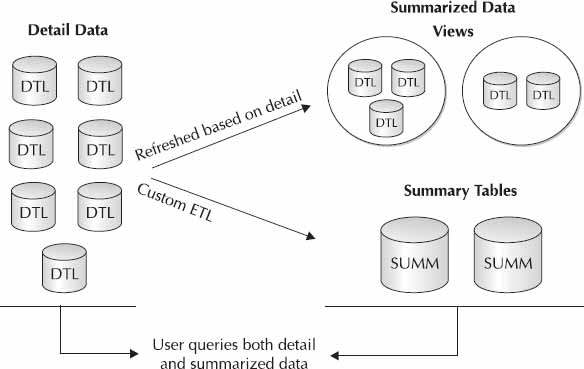
\includegraphics[width=0.5\textwidth]{FIG1}
    \caption{Summarization using views and summary tables}
    \label{fig_21}
\end{figure}
\\
\begin{figure}[ht!]
    \centering
    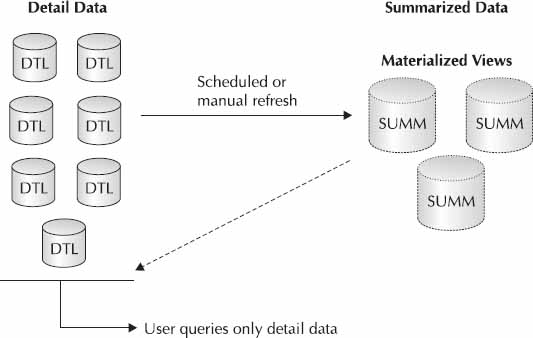
\includegraphics[width=0.5\textwidth]{FIG2}
    \caption{Summarization using materialized views}
    \label{fig_21}
\end{figure}
At this point, you may be asking yourself: “How do I determine what materialized views to create and at what level of summarization?” Oracle Database 12c has some utilities to help. These utilities are collectively called the SQL Tuning Advisor and will recommend materialized views based on historical queries, or based on theoretical scenarios. They can be run from the Oracle Enterprise Manager (OEM) Grid Control, or by calling the dbms advisor package.
\clearpage
\cleardoublepage

%CAPITOLUL3
%\section{Practical part}
\phantomsection
\lstinputlisting[style=mystyle, language=SQL, caption={Views creating statements},]{sourcecode/Create_Parameter_View_Oracle.sql}


For practical part, I will go step by step on this topic, will create the view, update it and then drop it in the end. Views can be used to reduce the complexity of the database schema, used as a mechanism to implement row and column level security and can be used to present aggregated data and hide detailed data.\\
 To begin, let's define 2 tables with data, from whom we will create our views. 
\begin{figure}[ht!]
    \centering
    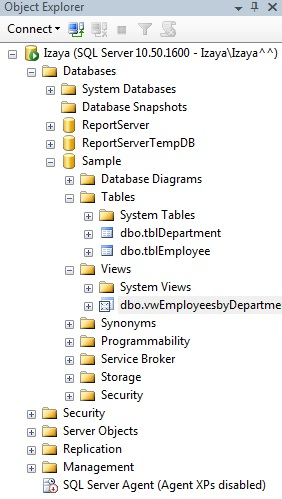
\includegraphics[width=0.5\textwidth]{CreateViewQuerySource}
    \caption{Project's Objects Explorer}
    \label{fig_21}
\end{figure}

As we can observe, we have 2 tables:
- tblDepartment (containing names of departments and their IDs)
- tblEmployee (containing all the information about the employees)
\\
Employee table will have 5 columns (ID, Name, Salary, Gender, DepartmentName)
and we will operate first of all by merging two tables, after this we will create a view. (note: by convention it is a good experience to start view names with vW)\\

\begin{figure}[ht!]
    \centering
    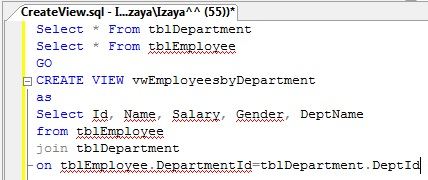
\includegraphics[width=0.5\textwidth]{CreateViewQuery}
    \caption{Creating View Query}
    \label{fig_21}
\end{figure}

Views simplify our work presenting the database for non-IT users, making it a lot more easier to generate, to manage accesses or to hide confidential data.
For our two tables, I will try to make different views for different kind of requests we'll get. \\
Let's give a specific table for someone who wants to join IT department and want to know his future co-workers:
\lstinputlisting[style=mystyle, language=SQL, caption={Views creating statements},]{sourcecode/PP_ITDep.sql}
So that's how the query will look like and the result will be this:
\begin{figure}[ht!]
    \centering
    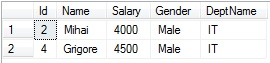
\includegraphics[width=0.5\textwidth]{ITDep}
    \caption{ITDepartment Query Result}
    \label{fig_21}
\end{figure}

In the Object Explorer we can see how we slowly add views in the Views Folder to the Sample Database that we are working in.
\begin{figure}[ht!]
    \centering
    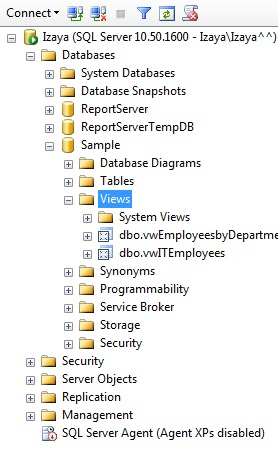
\includegraphics[width=0.5\textwidth]{ITDepSource}
    \caption{ITDepartment Query Result}
    \label{fig_21}
\end{figure}

Let's simulate the situation when we are publishing the database to all the employees or to third party. This is the case when some information from the table must be hide in order to protect status and behavior of the person.
For such a cases Views are a powerful tool that allows us to create a view from a table which will not contain the disturbing or personal information.
This is shown below:\\
\begin{figure}[ht!]
    \centering
    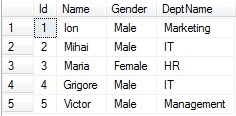
\includegraphics[width=0.5\textwidth]{NonConfidential}
    \caption{ITDepartment Query Result}
    \label{fig_21}
\end{figure}
As we can see, with a simple query I eliminated the column in which where the Salary of the employees by creating a view without this column, so the main table still holds this info, but for public eyes it is hiden.
\lstinputlisting[style=mystyle, language=SQL, caption={Views creating statements},]{sourcecode/PP_NonConfidential.sql}
\textbf{Update} for a view is done simply with clause Update and Set. In the following example I will change the name of a specific employee with a specific ID using Update clause. 
\begin{figure}[ht!]
    \centering
    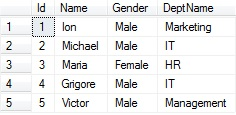
\includegraphics[width=0.5\textwidth]{Update}
    \caption{Updated View}
    \label{fig_21}
\end{figure}

Let's not forget that Views are also tables, and we can do things like deleting from a row or specific element, or to insert in a specific place our new data if it's free to insert.\\
\textbf{Deleting} a view is done by the command Drop, which performs in the following way:\\
\lstinputlisting[style=mystyle, language=SQL, caption={Views creating statements},]{sourcecode/Drop_viewCode.sql}
\begin{figure}[ht!]
    \centering
    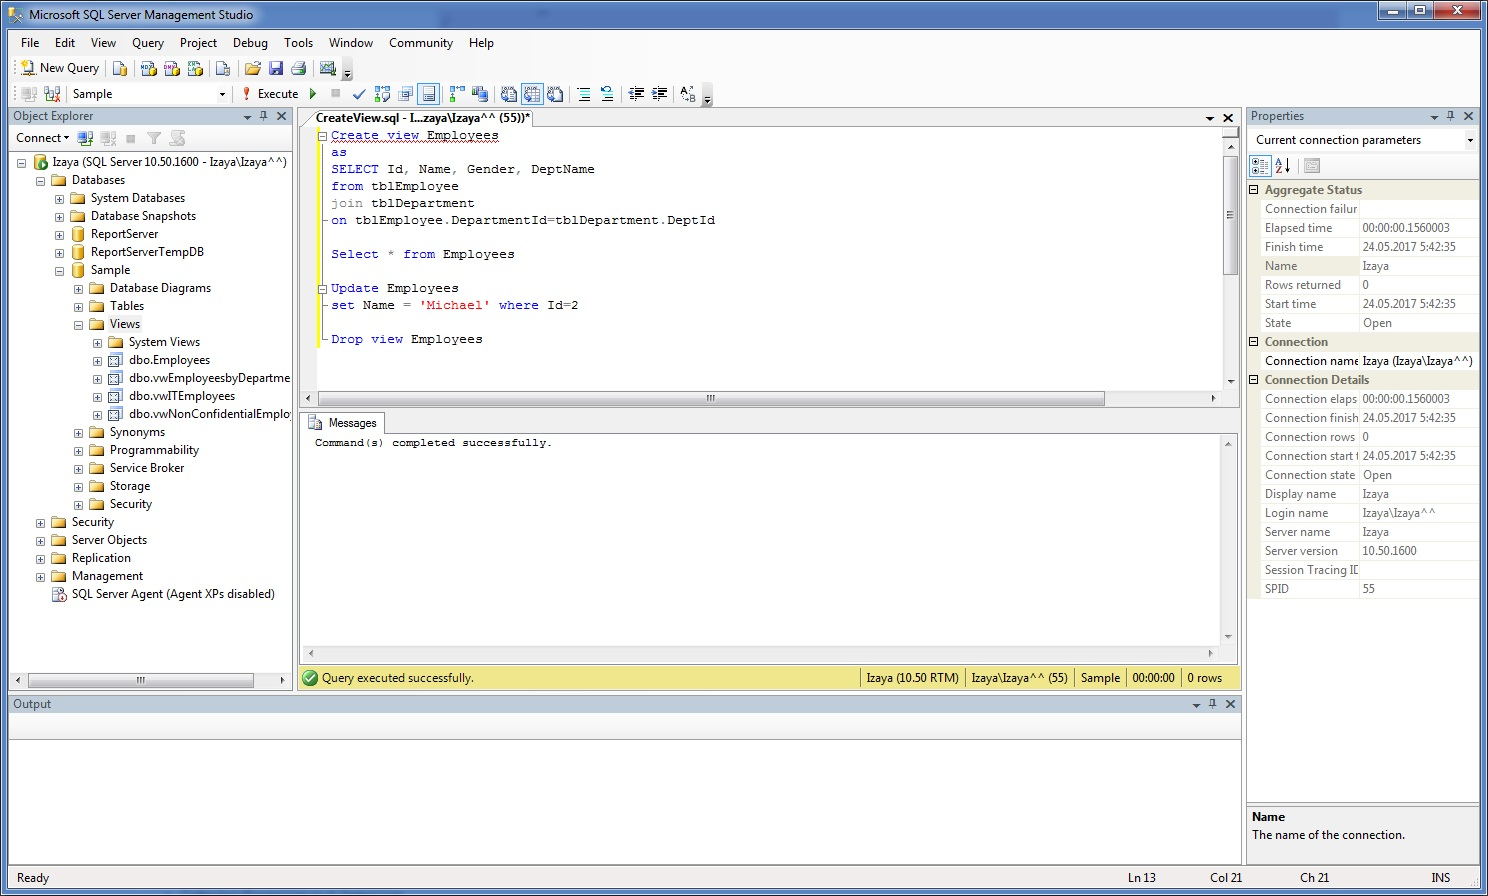
\includegraphics[width=0.5\textwidth]{DropView}
    \caption{Updated View}
    \label{fig_21}
\end{figure}

After we execute the DROP command we should see the elimination of the view in the Views folder of the project.\\
\begin{figure}[ht!]
    \centering
    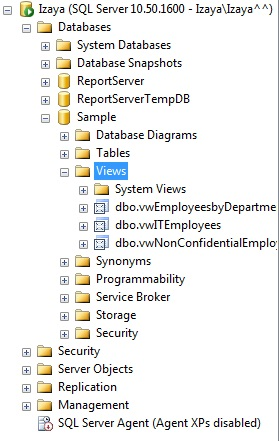
\includegraphics[width=0.5\textwidth]{DropViewAfter}
    \caption{Updated View}
    \label{fig_21}
\end{figure}

In such a simple way Views can facilitate work using simple query requests.
\clearpage
%\cleardoublepage


% IMPORTANT REMARK  
% If your table of contents need to be splitted in two parts (in order to accomodate the frame used for TOC)
% within the body text, right before the chapter/section that you want to be started on anew page, 
% you should add:     \addtocontents{toc}{\protect\newpage}

%CONCLUZII
\phantomsection
\addcontentsline{toc}{section}{Conclusions}
\section*{Conclusions}
\phantomsection


Views in SQL are a powerful tool that can simplify the work of the database architect or developer. By combining multiple tables in one view, easily updating and deleting some rows is facilitating the work and makes it a lot easier than using typical update and insert commands directly in the table of work. Views are statements with a name associated to it and stored in the database, this allows an easy creation and drop of the view in any moment of work. Depending on the type of view we need to use, the specific attributes should be modified in views. Views are virtual tables that facilitate the work for an IT person using a simpler way to give information and it can be used in different ways. From my opinion, views has 3 main functions, to reduce the complexity of the database schema, to implement higher row and column levels of security and to present aggregated data and hide detailed data.
The way how easy it is to create, update or delete a view we can exclaim that it is a tool that should be used more often and implemented on different databases.

\clearpage
\cleardoublepage

\cleardoublepage
\addcontentsline{toc}{section}{References}
\begin{thebibliography}{99999}
\phantomsection
\singlespace\normalsize

\bibitem{NaoOfficial} Aldebran Robotics, \textit{ official page}, \url{www.aldebaran.com/en}

\bibitem{doc} Aldebran Robotics, \textit{NAO Software 2.1.3 documentation}  \url{www.doc.aldebaran.com/2-1/index.html}

\bibitem{OC} OpenCV Dev Team, \textit{OpenCV 2.4.9.0 documentation}, \url{www.opencv.org/modules/refman.html}

\bibitem{Ojala} Timo Ojala, \textit{Multiresolution gray-scale and rotation invariant texture classification with local binary patterns}, 2002

\bibitem{Solem} Jan Erik Solem, \textit{Programming Computer Vision with Python}, 2012

\bibitem{FRUE} M. A. Turk and A. P. Pentland, \textit{Face Recognition Using Eigenfaces}, 1991.

\bibitem{SKK}S. Suhas, A. Kurhe, Dr.P. Khanale, \textit{Face Recognition Using Principal Component Analysis and Linear Discriminant Analysis on Holistic Approach in Facial Images Database}, Vol. 2, December 2012

\bibitem{Chellappa} W. Zhao, R. Chellappa, P. J. Phillips and A. Rosenfeld, \textit{Face recognitions literature survey'}, ACM Computing Surveys, Vol. 35, No. 4, December 2003, pp. 399–458

\bibitem{} Sukhan Lee, Hyungsuck Cho, Kwang-Joon Yoon, Jangmyung Lee, \textit{Intelligent Autonomous Systems 12}, Volume 1

\bibitem{Ismail} Shah Alam, Malaysia Shamsuddin, \textit{Face detection technique of Humanoid Robot NAO for application in robotic assistive therapy}, Center of Excellence for Humanoid Robot Bio-Sensing (HuRoBs), Univ. Teknol. MARA

\bibitem{ES1} Xavier Alameda-Pineda, Vasil Khalidov, Radu Horaud and Florence Forbes, \textit{Finding Audio-Visual Events in Informal Social Gatherings}

\bibitem{ES2}Jan Cech, Ravi Mittal, Antoine Deleforge, \textit{Active-Speaker Detection and Localization with Microphones and Cameras Embedded into a Robotic Head}, Humanoids 2013 - IEEE-RAS International Conference on Humanoid Robots, Oct 2013, Atlanta, United States. 2013

\bibitem{ES3} Xavier Alameda-Pineda, Radu Horaud, \textit{Vision-Guided Robot Hearing}, The International Journal of Robotics Research, SAGE Publications (UK and US), 2015


\end{thebibliography}

\cleardoublepage
   
 
\end{document}